\documentclass[9pt,onecolumn,oneside]{osajnl}
%% Please use 11pt if submitting to AOP
\usepackage{pgfplots}
\usepackage{graphicx}
\usepackage{hyperref}
\journal{ol} % Choose journal (ao,jocn,josaa,josab,ol,optica,pr)

%See template introduciton for guidance on setting shortarticle option
\setboolean{shortarticle}{false}
% true = letter/tutorial
% false = research/review article
% (depending on journal)



\title{Capturing the barycenter of a convex bi-dimensional shape with random points using computational algorithms}


\affil[1]{Mathematics EE, Sevenoaks School, High St, Sevenoaks TN13 1HU, United Kingdom}

\affil[*]{Corresponding author: teodor@calin.ro}



\begin{document}

\maketitle



\section{Introduction}

Problem A-6 of the 53rd Putnam Competition read as follows:

	“Four points are chosen at random on the surface of a sphere. What is the probability that the centre of the sphere lies inside the tetrahedron whose vertices are at the four points? (It is understood that each point is independently chosen relative to a uniform distribution on the sphere.)”(53rd Putnam, 1992, \url{https://prase.cz/kalva/putnam.html})
    
    This paper will approach a way of generalising and attempting to use complex algorithms for any bi-dimensional shape convex shape. The algorithms and software used will be described more thoroughly throughout the paper.


\section{Software used}

	The software used for calculating the probabilities is MATLAB. Custom software was also developed in order to generate the random shapes used during testing and data collection. The software was written in Javascript as various open-source libraries under the MIT license were available. These libraries were used for generating the bi-dimensional shapes and exporting the paths of the shapes in .SVG format. The paths were then imported into MATLAB. A Tensorflow Model(Convolutional Neural Networ) was also constructed, trained and implemented in the software developed which had the purpose of calculating the ‘similarity’ of the shape to a circle using Tensorflow and Python. The process will be further explained in the following sections of the paper.
    I posses knowledge in using these programming languages and these frameworks, reason why I picked them. Some of the choices made, such as using Python were sub optimal, due to the processing inefficiency. Even so, learning R, which would've been the optimal solution would take too much since it's completely different to anything I've done before.
 

\section{Methodology}

	A software solution was developed for generating the random convex bi-dimensional shapes. As mentioned before the programming language used was Javascript. The algorithm used for this process was the Graham Scan Convex Hull Algorithm. The path is then exported as an .SVG file that is ready to be processed in MATLAB. I chose this algorithm since it's really effective while being very simplistic overall. This helps as it allows for thousands of shapes to be generated every second. 

	The file would then be imported in MATLAB, then, 3 points,  \(P_{1}, P_{2}\)  and \(P_{3}\) are picked randomly on the perimeter of the shape by the MATLAB algorithm. If the the barycenter O is contained within the triangle \(T\) formed by the three points then the the triangle is added to , this is further described in the section "MATLAB Probability Calculation". The points are picked at a resolution of \( 10^{-12}\) of the perimeter of the shape until all the possibilities are exhausted.  The probability was calculated by dividing the number of triangles that captured the barycenter within their area and the total number of triangles constructed by the computer algorithm. The similarity of the shape to a circle is also noted after running the .SVG through the Tensorflow model. All this data would be entered in a table and observations would be drawn.

\subsection{Shape Generation Algorithm}

	The following Algorithm is used to generate the shapes used in the experiment. This algorithm is applied to a series of points generated by a random number generator. 

\begin{algorithm}
\caption{Graham Scan Convex Hull algorithm}
\begin{algorithmic}[1]
\State{Let N}\Comment{Number of points}
\State{Let Points[N+1]} \Comment{Array of points}
\State{Swap Points[1] with the point with lowest y-coordinate}
\Comment{We want points[0] to be a sentinel point that will stop the loop.}
\State{Sort Points by polar angle with Points[1]}
\State{Let points[0] = points[N]}
\State{Let M = 1}
\Comment{M will denote the number of points on the convex hull.}
\For{i = 2 to N:}
	\Comment{Find next valid point on convex hull.}
    \While{ccw(Points[M-1], Points[M], Points[i]) <= 0}
        \If{M > 1:} 
            \State {M -= 1}
            \State {\emph{continue}}
            \Comment{All points are collinear}
        \EndIf
        \If{i == N:}
            \State {\emph{break}}
            \Comment{Reached the number of desired points, exit loop}
        \EndIf
        \State i+=1
        \Comment{Increment variable i by 1}
    \EndWhile
\EndFor
\State M+=1
\State{Swap Points[M] with Points[i]}
\Comment{Update M and swap points[i] to the correct place.}
\end{algorithmic}
\end{algorithm}

	The result of this algorithm is an array of points with the corresponding coordinates in the order that constitutes a convex bi-dimensional shape S. Below is also some diagrams( \textbf{Fig. 1., Fig. 2., Fig. 3., Fig. 4.}) exemplifying how this algorithm works, or more specifically a couple of steps in the choosing of points: 

\[Points[N] = P_{0}, P_{1}, P_{2}, ... , P_{N}\]
\[P_{N} = (x_{N}, y_{N}) \]



\begin{figure}[h]
  \centering
  \begin{minipage}[b]{0.18\textwidth}
  	\centering
    \includegraphics[width=\textwidth]{2.png}
    \caption{Step n}
  \end{minipage}
  \hfill
  \begin{minipage}[b]{0.18\textwidth}
  	\centering
    \includegraphics[width=\textwidth]{1.png}
    \caption{Step n+1}
  \end{minipage}
  \hfill
  \begin{minipage}[b]{0.18\textwidth}
  	\centering
    \includegraphics[width=\textwidth]{3.png}
    \caption{Step n+2}
  \end{minipage}
  \hfill
  \begin{minipage}[b]{0.18\textwidth}
  	\centering
    \includegraphics[width=\textwidth]{4.png}
    \caption{Final step}
  \end{minipage}\\
  \textit{Source: "\url{https://en.wikipedia.org/wiki/Graham_scan}"}
 \end{figure}

	\(Points[N]\) determines a unidimensional matrix, also called vector in computer science. It's basically a unidimensional array with data that is accessable from the index. In my case this was the preffered way of formatting the data since it's very convenient. To put it in perspective, if I would want to access the 5th point,  I would simply have to call \(Points[5]\), which would return me the value of the 5th point.
    
    I have also added a small demonstration of this algorithm on my github, publicly visible. It generates a number of points randomly and calculates the convex hull for those points. It is accesable through this link: \url{https://teoslayer.github.io/Graham/index.html}



\subsection{MATLAB Probability Calculation}

	Let points \(P_{1}, P_{2}, P_{3} \subset S\). Let point \(O\) = barycenter of shape \(S\). Let \(T\) = Triangle determined by points \(P_{1}, P_{2}, P_{3}\). The three points are chosen at random on the perimeter \(X\) of shape \(S\) at increments of \(X/{10^{12}}\). A number of \(N\) runs are completed. Let \(A\) be the set of all triangles. The probability of  \(T\) to capture the barycenter is determined by the equation below:

\[A = \{T_{1}, T_{2}, T_{3}, ..., T_{N}\}\]
\[Probability = \frac{n(O \subset T |   \forall T  \in A)}{N}\]
	The equation above describes the number of the triangles of which the barycenter \(O\) is included\((\subset )\) within the bounds of the Triangle \(T\). The software program written in MATLAB is able to determine the inclusion based on the coordinates of the barycenter \(O\). If the coordinates of barycenter O intersect the area of the triangle T then the triangle is marked as valid. The equation above states the following:
The probability is equal to the total amount of elements of the set where \(O\) is included in \(T\) for every\((\forall )\) \(T\) included\((\in)\) in set \(A\) divided by \(N\), which can also be expressed as \(n(A)\), where \(N\) is the cardinal number(total amount of elements in the set) of set \(A\) or the total amount of runs.

\subsubsection{Computational Concerns}

	The most concerning thing about this probability calculation was the resolution necessary for calculating a "precise" result. Initially I started off with increments of \(1/10^{18}\) . A single run took about 1 minute to run. This may not look like a lot but by multiplying that minute with the literal billions of files I had to process it started worrying me. A single billion of files would mean approximately 1903  years. I started tuning down the resolution by increments of \(10^{3}\). With increments of \(1/10^{15}\), it would only take 5 months to compute one billion files. My only guess that the big time jump was due to the fact that I could use data types which occupied less memory and thus could be computed faster. With \(1/10^{12}\), I reduced the time necessary to only 5 days for one billion files. I have to specify that this was when I was testing it using my home computer. In the end I managed to acquire a computer that was more powerful than mine which further reduced the time to approximately 0.8 days or about 19 hours. This resolution difference produced inconsistencies in the orders of magnitude of \(10^{-4}\) which I considered acceptable considering the time necessary to process all the data.
    


\subsection{The Tensorflow Model}


	Knowing the result to the initial Putnam question\((\frac{1}{4})\) I made the presumption that an algorithm to determine the similarity of the shape to a circle would play an important role. Since creating a mathematical model from scratch is beyond my mathematical knowledge I decided to make an approach that would be in my domain of knowledge. So, as a result, I decided to build a Neural Network Model. The architecture used for developing this Model is CNN, Convolutional Neural Network or ConvNet. The choice was done due to the possibility of developing ‘feature learning’ throughout testing and execution. This way the algorithm would behave more like a recursive neural network, learning not only through training but also during testing runs. Also ConvNet allows for more data dimensions than a regular neural network. This allows us to work with bi-dimensional matrices, which in our case would be the actual .SVG shapes. These would be broken down in pixels and interpreted as a bi-dimensional matrix. In a conventional neural network the input bi-dimensional matrix of the shape had to be converted into a uni-dimensional matrix. Due to the size of the bi-dimensional matrix, we would be creating a uni-dimensional matrix which would be too large, making training and testing almost impossible.

	 The .SVG file was flattened and broken down into \(6.25 \times  10^{6}\) Segments these were then run through the first Kernel Convolution Process(\(n1\)), with \(h\), a \(5\times5\) matrix. The Kernel shifts, performing matrix multiplication operations between \( h\) and portions of the input matrix \(f\) to give us a Convoluted Feature Output. The output of the first Kernel shift is then run through multiple Max Pooling layers and other Kernel shifts as we go through the flow, as described in the \(Architecture\) section. At the last channel(\(n3\)) we get a tensor with the size of \(4 \times 4 \times n3\). This is then flattened into a uni-dimensional matrix that can be easily interpreted by a Conventional Neural Network. The neural network has \(2\) other abstraction layers of \(50\) nodes, \(n4\) and \(n5\). The output of the neural network gives us a floating output between \(0.01\) and \(0.95\), more specifically the similarity of the shape to a circle ( \(C\) ). The process, including the definitions and namings, are further described in the following sections.
 
\subsection{Convolution Process}

	Kernel convolution is an important process of many computer vision algorithms. The process itself is named from the small matrix of numbers, called kernel, which is passed over our matrix \(f\), transforming it based on the numerical values within the kernel \(h\). The process is done with the formula below, where \(m\) and \(n\) are the indexes of rows and columns and \(f\) and \(h\) are the input matrix and the kernel respectively. The variables \(j\) and \(k\) represent the vertical and horizontal indexes on the kernel.
 \[G[m, n] = (f * h)[m, n] = \sum_{j}\sum_{k}h[j,k]f[m - j, n - k]\]



 The input matrix, \(f\), for the shape broken down in pixels 2500 \times 2500 is as follows:
 


\[
f =\begin{bmatrix}
a_{1,1} & a_{1,2} & a_{1,3} & a_{1,4} & a_{...} & a_{1,2500}\\
a_{2,1} & a_{2,2} & a_{2,3} & a_{2,4} & a_{...} & a_{2,2500}\\
a_{3,1} & a_{3,2} & a_{3,3} & a_{3,4} & a_{...} & a_{3,2500}\\
...\\
a_{2500,1} & a_{2500,2} & a_{2500,3} & a_{2500,4} & a_{...} & a_{2500,2500}
\end{bmatrix} \]



	For each element in the matrix, \(a_{m,n} \) we can either have a value of \(0\) or \(1\), where \((m,n)\) are the indexes of rows and columns. The value of each element is denoted by the binary pixel value extracted from the shape file. If the segment contains any pixels then it gets the value of 1, if it doesn't, it gets the value of 0.

	The Kernel, \(h\), used during our transformations/convolutions, is a \(5*5\) matrix with the values below:

\[h =\begin{bmatrix}
1 & 0 & 0 & 0 & 1\\
1 & 0 & 0 & 0 & 1\\
1 & 0 & 0 & 0 & 1\\
1 & 0 & 0 & 0 & 1\\
1 & 0 & 0 & 0 & 1
\end{bmatrix} \]
  The Kernel \(h\), shift along the whole matrix, performing the equation specified above. Kernel padding is also applied, meaning that the Kernel doesn't get out of the bounds of the matrix \(f\) and doesn't overlap with other kernels. After the process is done we get a convoluted feature output, \(
\alpha\) as a result. This is a smaller matrix than the initial matrix that presents the same features as the input matrix. This essentially scales down our initial matrix size by \(\frac{1}{5}\) after every convolution process, lowering the overall resolution of the matrix but maintaining the same patterns. This can be observed in the diagram shown in the "Architecture" section. After the first convolution process(Conv\textunderscore1) our matrix is reduced from a size of \(2500 \times 2500 \) to a matrix of \(500 \times 500\) while keeping the same features of the input matrix. Below I have presented an example including a diagram(\textbf{Fig. 6.}), the input matrix in the diagram, the kernel and the resulting output.
    
    \begin{figure}[h]
  \centering
  \begin{minipage}[b]{0.9\textwidth}
    \includegraphics[width=\textwidth]{kerneling.png}
  \end{minipage}
  \text{\textbf{Fig. 5.} Sobel Function Demonstration}\\
\end{figure}

\begin{figure}[h]
  \centering
   \begin{minipage}[b]{0.3\textwidth}
  \[f =\begin{bmatrix}
10 & 10 & 10 & 10 & 10 & 10\\
10 & 10 & 10 & 10 & 10 & 10\\
10 & 10 & 10 & 10 & 10 & 10\\
0 & 0 & 0 & 0 & 0 & 0\\
0 & 0 & 0 & 0 & 0 & 0\\
0 & 0 & 0 & 0 & 0 & 0
\end{bmatrix} \]
  \end{minipage}
  \hfill
  \begin{minipage}[b]{0.3\textwidth}
  \[h =\begin{bmatrix}
1 & 2 & 1\\
0 & 0 & 0 \\
-1 & -2 & -1
\end{bmatrix} \]
\end{minipage}
\hfill
\begin{minipage}[b]{0.3\textwidth}
  \[\alpha =\begin{bmatrix}
0 & 0 & 0 & 0\\
40 & 40 & 40 & 40 \\
40 & 40 & 40 & 40 \\
0 & 0 & 0 & 0
\end{bmatrix} \]
\end{minipage}
  \hfill
  
 \end{figure}\\


    
    Below I have also provided a more visual example(\textbf{Fig. 5.} of how convolution works on an image in a top Sobel convolution function. This is an operator used in image processing neural networks, mostly used in edge detection cases. The kernel for the Sobel Function or more specifficaly the Sobel Operator is:\\
    
    \[h =\begin{bmatrix}
1 & 2 & 1\\
0 & 0 & 0 \\
-1 & -2 & -1
\end{bmatrix} \]
\begin{figure}[h]
  \centering
  \begin{minipage}[b]{0.9\textwidth}
    \includegraphics[width=\textwidth]{sobel.png}
  \end{minipage}
  \text{\textbf{Fig. 6.} Sobel Function Demonstration}\\
  \textit{Source: "\url{https://setosa.io/ev/image-kernels/}"}
\end{figure}

	In the image below(\textbf{Fig. 5.} the kernelling applied to the input image sweeps across the whole matrix(image pixel values) sequentially, resulting the output matrix, or in our case the output matrix. The only difference between my process and this example is that here the convoluted feature output(\(\alpha\)) is the same size as the input matrix. This is because in the sobel transformation the segments of the matrix overlap while in our process it doesn't, similarly to how max pooling works. This is further explained in the next section. This way we further reduce the complexity of our matrix without performing more max pooling operations. 
  

\subsection{Max Pooling Process}

	In order to further simplify our matrix before running it through the conventional neural network we also go through a process called max pooling. This is done by transforming the matrix by selecting various segments and extracting the maximal value of the segment.

	Example 1:

	We perform max pooling, with segments of \(2\times2\), \(\beta_{n}\), where \(\beta\) is the segment that we're currently processing.

\[f =\begin{bmatrix}
30 & 10 & 15 & 38 & 10 & 10\\
10 & 20 & 10 & 10 & 22 & 10\\
10 & 10 & 10 & 18 & 10 & 10\\
0 & 0 & 0 & 0 & 0 & 0\\
0 & 0 & 0 & 0 & 0 & 0\\
0 & 0 & 0 & 0 & 0 & 0
\end{bmatrix} \]
	The segment, \(\beta_{1}\), in our case would be:

\[\beta_{1} =\begin{bmatrix}
30 & 10\\
10 & 20\\
\end{bmatrix} \]
	The maximum value in \(\beta_{1}\)would be \(30\). Following the same procedure, by shifting across the whole matrix we get the following matrix, \(\alpha\). An important aspect of the max pooling process is to prevent overlapping of the segments. Below you can find the output matrix and a graphic illustration:



\[\alpha =\begin{bmatrix}
30 & 38 & 22\\
10 & 18 & 10\\
0 & 0 & 0
\end{bmatrix} \]
\begin{figure}[h]
  \centering
  \begin{minipage}[b]{0.5\textwidth}
  	\centering
    \includegraphics[width=\textwidth]{max-pooling.png}
    \text{\textbf{Fig. 7.} Max Pooling Matrix Segmentation}
  \end{minipage}
\end{figure}

	In the image and matrix above the result of the max pooling process can be observed. The input matrix is essentially broken down into multiple matrices with the size we determined( red segments ). The output matrix \(\alpha\) will be equal to a matrix the size of the horizontal and vertical number of segments( in our case a \(3 \times 3\) matrix) with the corresponding values of the maximal values in the segments (highlighted with green). This is usually done using the \(max()\) function below:
    
    \[max(a,b)=\frac{1}{2}(a+b+|a-b|)\]
  This is done sequentially between values present in the segments until the maximal value is obtained. 
For example in our case in \(\beta_{1}\), we would first apply \(max(a_{1,1},a_{1,2})\)(\(\max(30,10)\)), then the result of that is applied in the next \(max()\) function with the next element, and so on and so forth until we have cleared the whole segment. Then we proceed to the next segment until we fill the whole matrix.

	Overall this has the purpose of reducing the size of the matrix while still retaining some of the features in the input matrix. This is done in order to reduce the computational power necessary while still keeping some of the patterns observed in the initial matrix.
    
    
\pagebreak
\subsection{Neural Network}

	Neural networks are digital interpretations of natural neural networks. They are composed of 2 basic elements: nodes and connections. The natural counterparts to these two elements are neurons and synapses. Sometimes when working with digital neural networks nodes can also be called neurons. Every node has inputs and outputs just like neurons have axons and dendrites. A neuron works by computing the inputs with a certain activation function \(f\) and return a certain output which it passes on to other neurons or to the user as raw data. 
    

    
    \begin{figure}[h]
      \centering
      \begin{minipage}[b]{0.6\textwidth}
        \centering
        \includegraphics[width=\textwidth]{neuron.png}
        \text{\textbf{Fig. 8.} Neuron}\\
         \textit{Source: "\url{https://ujjwalkarn.me/2016/08/09/quick-intro-neural-networks/}"}
      \end{minipage}
    \end{figure}

	In our case the activation function \(f(x)\) is a ReLU(Rectified Linear Unit) activation function. The function is defined as follows:
    
    \[{\displaystyle f(x)=x^{+}=\max(0,x)=\frac{1}{2}(x+0+|x-0|)}\]
    
    Essentially the function is simply a way to filter off negative values. Any negative input gives a null output(\(0\)). The parameter \(x\) applied to the function is a sum of all inputs which are multiplied to a parameter called weight(\(w\)) and a parameter called bias, \(b\). The bias is a constant attributed to the neuron which shifts the input \(x\) applied to function \(f(x)\) without adjusting the weights of the inputs. In some cases where \(x\) might be negative this can help offset \(x\) so the output of the function won't be \(0\).
    
    For example in this case the neuron has 2 inputs: \(X1\) and \(X2\). Let's consider the weight for input \(X1\) , \(w1\), as \(0.6\) and the weight for input \(X2\) , \(w2\),  as 0.8 and bias \(b\) as 0.6. Let's consider both \(X1\) and \(X2\) as having values of \(1\). By computing the function \(f(x)\) we get the following:
\[x = X1 * 0.6 + X2 * 0.8 + 0.6\]
\[ x = 1 * 0.6 + 1 * 0.8 + 0.6 \]
\[x = 2\]
\[f(x) = \max(0,2)\]
\[f(x) = \frac{1}{2}(2+0+|2-0|) \]
\[ f(x) = 2\]
	Thus the output of this neuron, with the predetermined parameters listed above, is 2. By combining these nodes in various combinations and layers you can obtain a complex network of equations with parameters you can vary to fit your desired output. This is called a  neural network. Neural networks are composed of 3 important domains: the input domain, the hidden layers and the output. The input domain is usually composed of a layer of input neurons. These take the input data and process them using the activating function \(f\), but have a bias \(b\) of 0. In my case I have a layer of 25 neurons as inputs. The hidden layers are composed of various layers of neurons of various sizes. These are called hidden layers because the variables and connections are not directly visible by the user that sets up the neural network. It's basically considered as a layer of abstraction between the Input and Output. In my case I have 2 hidden layers\((n4, n5)\) with 25 neurons each. The output consist of a number of neurons which give us the final desired value. In my case I only have 1 output neuron which gives me the final value \(C\), the similarity of the shape \(S\) to a circle. The Architecture Diagram of the Neural Network can be seen in \textbf{Fig. 8}.\\
    
  

  Coming back to the example above, of course, you can calculate the weights and biases yourself. Unfortunately this is not how neural networks are set up. The typical way these values are calculated is through a variation of "brute force", or more specifically by going through all the possible values to obtain the desired output for the predetermined input. This is called \textbf{Training}. In our case I have a collection of .SVG files of circles/ovals and various other shapes. For each set of data we attribute a certain value to the output. Then training software is executed, which mix the connections, weights and biases in the hidden layers until we get the desired output. This usually requires huge amounts of data, hence the large number of files used during training.\\
  
    \begin{figure}[h]
  \centering
  \begin{minipage}[b]{0.6\textwidth}
  	\centering
    \includegraphics[width=\textwidth]{nn.png}
    \text{\textbf{Fig. 9.} FC\textunderscore4 Neural Network}
  \end{minipage}
\end{figure}
  
    
    
\subsubsection{Training and Testing}  

	In order for my model to not become biased towards circles 2 training phases were done. Sometimes if you use only one type of data the model can become biased. For example if you create a model that identifies vehicles and you only present it images of cars it will become biased towards cars. If you present it any other vehicle, such as a motorcycle, it won't identify it as a vehicle. In my case, in the first phase I'll present it images of circles and in the second phase images of ovals.\\

\emph{Phase 1}\\

	Initially, the model was trained using .SVG files of circles, which were attributed a value of \(0.95\) to \(R\), the desired output. Three training runs were done involving this strategy. This would lead to the abstraction layers\((n4, n5)\) to always give an output of \(0.95\) when presented paths of circles. This phase involved \(10^{12}\) .SVG files of circles.\\

\emph{Phase 2}\\

	Phase 2 involved training with .SVG files of ovals, which were attributed a value of \(0.9\) to \(R\). Another three training runs were done, which resulted in the abstraction layers giving outputs between \(0.85\) and \(0.9\). This phase involved \(10^{8}\) .SVG files of ovals with varying distances between the two focal points.\\

\emph{Testing}\\

	The testing phase was the first time the model was presented shapes that differed from ovals or circles. The shapes were generated by the script mentioned in the methodology section. As the model was trained to identify ovals and circles it resulted in promising values. As the testing was done manually it involved a small amount of shapes, approximately 80-90 shapes. The model was challenged by presenting various concave shapes or lines which resulted in values of 0.1 and 0.15. \\
    
    
    
\subsection{Architecture}


	By combining multiple convolution and max pooling layers, the matrix can be simplified but still retain some of the details of the initial matrix. This way I essentially get data that is simple enough to interpret into a conventional neural network(FC_4) while retaining high volumes of information. In my case I have applied 3 convolution layers with 2 max pooling layers, reducing the initial matrix from \(2500 \times 2500 \times 1\) to \(5 \times 5 \times n3\). This reduces the initial node count from \(6.25*10^{6}\) to just \(75\) nodes. The conventional neural network is composed of 2 more abstraction layers. which lead to the final node which returns a floating value \(C\) with values ranging from 0.1 to 0.95, the similarity of the shape to a circle.
        

\begin{figure}[h]
  \centering
  \begin{minipage}[b]{0.9\textwidth}
    \centering
    \includegraphics[width=\textwidth]{diagram.png}
    \text{\textbf{Fig. 10.} Architectural Diagram}
  \end{minipage}
\end{figure}



\section{Data Processing}

After the Training and Testing phase showed promising results I started doing the first run in order to finally obtain some data. I generated a set of files for the run, calculated the probabilities and then ran them through the model as explained in the methodology section.

\subsection{First Run}

	Below the results from the first run can be found. The run implicated \(10^{6}\) randomly generated shapes. 

\begin{table}[h!]
\centering
 \begin{tabular}{||c c c||} 
 \hline
 Circle Similarity( C ) & Avg. Probability( Pr ) & Count(\(+-0.001\) )\\ [0.5ex] 
 \hline\hline
 0.01 - 0.2 & 0.42 & \(1.475*10^{5}\)\\ 
 0.2 - 0.4 & 0.36 & \(2.348*10^{5}\)\\
 0.4 - 0.6 & 0.32 & \(2.992*10^{5}\)\\
 0.6 -  0.8 & 0.29 & \(2.101*10^{5}\)\\
 0.8 - 0.9 & 0.26 & \(1.006*10^{5}\)\\ 
 \hline
\end{tabular}
\end{table}

\begin{center}
\begin{tikzpicture}[h]
\centering
\begin{axis}[
    title={Avg. Probability to Circle similarity},
    xlabel={Circle Similarity (\(C)\)},
    ylabel={Average Probability \(Pr\)},
    xmin=0, xmax=1,
    ymin=0, ymax=45,
    xtick={0,0.1,0.2,0.3,0.4,0.5,0.6,0.7,0.8,0.9,1.0},
    ytick={0,5,10,15,20,25,30,35,40,45},
    legend pos=north west,
    ymajorgrids=true,
    grid style=dashed,
]

\addplot[
    color=blue,
    mark=square,
    ]
    coordinates {
    (0.05,43.2)(0.2,36.2)(0.4,33)(0.6,29.2)(0.8,26.3)(0.9,25.4)
    };
    \legend{Probability}
\end{axis}
\end{tikzpicture}
\end{center}



\subsubsection{Observations}

	From the graphs above we can determine that there is a strong linear correlation between the similarity of the shape to a circle, \(C\), and \(Pr\), the average probability of the triangle including \(O\) within its bounds. A trendline was also drawn giving us an equation that could be used to determine the probability by using C as a parameter.
    
    \[Pr = -0.178C + 0.4063\]
    It should also be observed that the distribution of Similarity across followed a normal distribution pattern. It’s possible that the Probability/Similarity graph did not follow a perfect linear path due to the random number generation algorithm.
    
	Further runs have to be done in order to confirm that this trend is in fact a trend and that the equation above is consistent across multiple datasets. In order to determine this I made two more runs, which seemed like a pretty fair number of runs.


\subsection{Second Run}

	Below the results from the second run can be found. The run implicated \(8.87*10^{6}\) randomly generated shapes. 

\begin{table}[h!]
\centering
 \begin{tabular}{||c c c||} 
 \hline
 Circle Similarity( C ) & Avg. Probability( Pr ) & Count(\(+-0.001\) )\\ [0.5ex] 
 \hline\hline
 0.01 - 0.2 & 0.43 & \(1.123*10^{5}\)\\ 
 0.2 - 0.4 & 0.37 & \(1.912*10^{5}\)\\
 0.4 - 0.6 & 0.33 & \(2.743*10^{5}\)\\
 0.6 -  0.8 & 0.31 & \(2.112*10^{5}\)\\
 0.8 - 0.9 & 0.27 & \(9.802*10^{4}\)\\ 
 \hline
\end{tabular}
\end{table}

\begin{center}
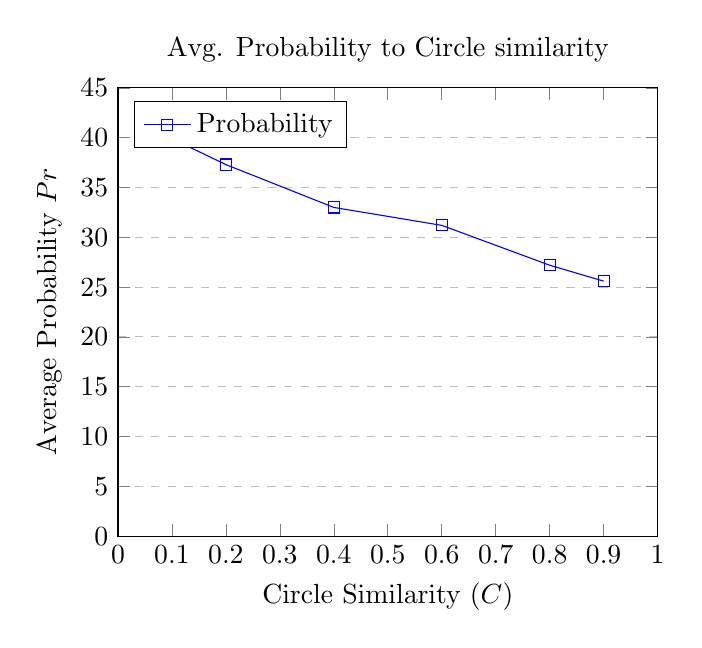
\begin{tikzpicture}
\centering
\begin{axis}[
    title={Avg. Probability to Circle similarity},
    xlabel={Circle Similarity (\(C)\)},
    ylabel={Average Probability \(Pr\)},
    xmin=0, xmax=1,
    ymin=0, ymax=45,
    xtick={0,0.1,0.2,0.3,0.4,0.5,0.6,0.7,0.8,0.9,1.0},
    ytick={0,5,10,15,20,25,30,35,40,45},
    legend pos=north west,
    ymajorgrids=true,
    grid style=dashed,
]

\addplot[
    color=blue,
    mark=square,
    ]
    coordinates {
    (0.05,41.2)(0.2,37.3)(0.4,33)(0.6,31.2)(0.8,27.2)(0.9,25.6)
    };
    \legend{Probability}
\end{axis}
\end{tikzpicture}
\end{center}


\subsubsection{Observations}

	In run 2 we can observe that the trendline equation is:
\[Pr = -0.1689C + 0.4085\]

\subsection{Third Run}

	Below the results from the third run can be found. The run implicated \(8.04*10^{6}\) randomly generated shapes. 


\begin{table}[h!]
\centering
 \begin{tabular}{||c c c||} 
 \hline
 Circle Similarity( C ) & Avg. Probability( Pr ) & Count(\(+-0.001\) )\\ [0.5ex] 
 \hline\hline
 0.01 - 0.2 & 0.41 & \(1.061*10^{5}\)\\ 
 0.2 - 0.4 & 0.39 & \(1.904*10^{5}\)\\
 0.4 - 0.6 & 0.35 & \(2.425*10^{5}\)\\
 0.6 -  0.8 & 0.32 & \(1.803*10^{5}\)\\
 0.8 - 0.9 & 0.28 & \(8.514*10^{4}\)\\ 
 \hline
\end{tabular}
\end{table}

\begin{center}
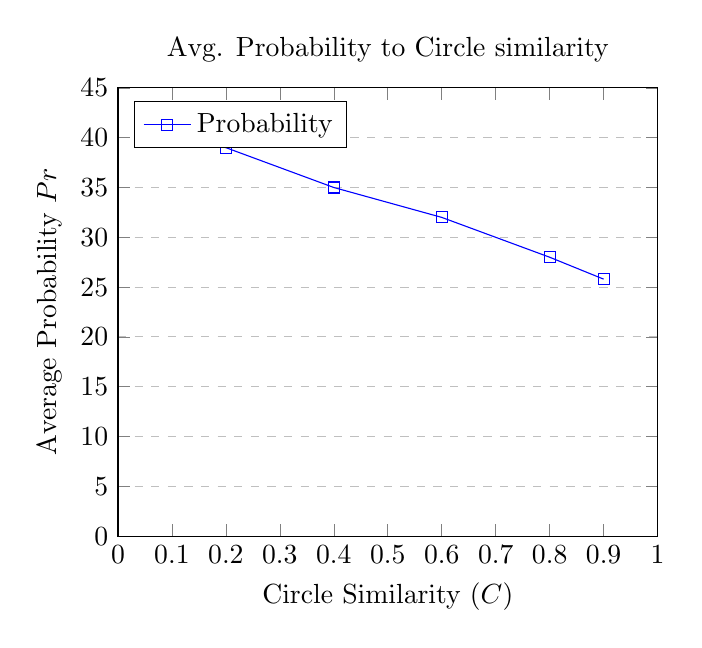
\begin{tikzpicture}
\begin{axis}[
    title={Avg. Probability to Circle similarity},
    xlabel={Circle Similarity (\(C)\)},
    ylabel={Average Probability \(Pr\)},
    xmin=0, xmax=1,
    ymin=0, ymax=45,
    xtick={0,0.1,0.2,0.3,0.4,0.5,0.6,0.7,0.8,0.9,1.0},
    ytick={0,5,10,15,20,25,30,35,40,45},
    legend pos=north west,
    ymajorgrids=true,
    grid style=dashed,
]

\addplot[
    color=blue,
    mark=square,
    ]
    coordinates {
    (0.05,41)(0.2,39)(0.4,35)(0.6,32)(0.8,28)(0.9,25.8)
    };
    \legend{Probability}
\end{axis}
\end{tikzpicture}
\end{center}

\subsubsection{Observations}

	In run 3 we can observe that the trendline equation is:
\[Pr = -0.1711C + 0.4205\]
	Taking in consideration all the runs we can fairly observe that the linear equation in question that determines the probability of the barycenter to be included within the bounds of the triangle determined by the 3 points is roughly:
\[Pr = -0.1726 * C + 0.4117\]
\section{Weaknesses}

	There are two main problems in the methodology that affected the precision of the equation. It can be easily observed that when computing the equation to a circle shape, where the result is \(1/4\), the result is fairly consistent but not completely precise . By plugging in the value for a perfect circle we get:

\[0.95 * ( -0.1726) + 0.4117 =~ 0.24773\]

	The first problem in the methodology is the resolution of choosing points. The resolution is not good enough to obtain a perfect answer. The decision to pick this exact resolution( Segments of \(10^{-12} * Perimeter\) ) was done due to computational and time limitations. The resolution can be increased but it would lead to longer times in checking each shape and thus it would take significantly more time to conduct the runs. A solution could be to reduce the sample size but this would also affect the precision of the run as there would be less data to work with. 
    
    The second problem was the process of breaking down shapes when computing the similarity to a circle ( \(C\) ). Since the .SVG files have to be broken down into matrices of \(2500\times2500\) the precision also gets affected. This effectively turns the .SVG file, which is a vector file, having essentially infinite resolution, into a normal image with a resolution of \(6.25\) megapixels. Even phone cameras have more resolution than this, the typical resolution being 12 megapixels. This may seem like enough but during the kernelling and max pooling of the initial matrix, further inconsistencies can appear which may affect the result before entering the neural network.

\section{Improvements}

	All the decisions that may have affected the precision of the results were done due to temporal or computational limitations. In order to execute the methodology described above and obtain more precise results either more computational power is required either more time is required. 
    
 \section{Conclusion}

	From the results of this paper a direct linear correlation between the probability of the barycentre to be captured within the bounds of a triangle determined by 3 points randomly chosen on a circle and the similarity of that shape to a circle can be observed. The methodology above showed promising results in how this could be executed by using specialised software. According to the algorithm implemented and the methodology described above, the equation that determines the probability is approximately:
    
    \[Pr = -0.1726C + 0.41397\]
    Where \(Pr\) is the probability, ranging from \(0\) to \(100\) and \(C\) being the similarity of the shape to a circle, ranging from \(0\) to \(0.95\).
    
  \cite{Pelt254}\cite{Wang2003}\cite{Kim2017}\cite{10.1145/3082031.3083236}\cite{5352485}\cite{80269}\cite{anthony1999neural}\cite{FEINDT2006190}\cite{8308186}
    

\bibliographyfullrefs{sample.bib}


\end{document}
